\section{Introduction}
Web users increasingly reach information through systems that decide what to retrieve before the user sees it. Search, recommendation, retrieval-augmented systems, and emerging agentic interfaces all depend on an initial selection of content. For a shopping agent to compare a relevant product, that product must first enter its candidate set. This motivates a retrieval question, without assuming that better retrieval necessarily improves recommendations or purchases: \emph{can irrelevant choices in how unchanged information is represented determine whether relevant content is found?}

Much of the Web is structured or semi-structured. Products, jobs, hotels, and events are stored as fields, yet neural retrieval often consumes flattened token sequences. Many underlying facts have no meaningful linear order. Product color, material, dimensions, and compatibility remain the same facts when their positions in a record change. This mismatch makes serialization a potential nuisance signal between semantic relevance and retrieval visibility.

E-commerce provides a controlled setting for studying that mismatch. We preserve product identity, all source facts, the query, the model, and the relevance labels while permuting complete attribute atoms. We distinguish a catalog-wide intervention, corresponding to a shared indexing change, from a target-only intervention that holds every competitor in its original representation. The latter supports the precise comparison: same product, same facts, same competitors, same query, same model; only the target serialization changes.

Figure~\ref{fig:example} illustrates the effect. For \emph{turquoise chair}, an Exact-relevant product moves between ranks 5 and 1,527 under different attribute orders with every competitor fixed. Its original rank is 486. The example is selected for interpretability and a large crossing; aggregate results, rather than this extreme case, establish the population pattern. The full title, source atoms, identifiers, and all tested ranks are included in the artifact and appendix.

\begin{figure}[H]
\centering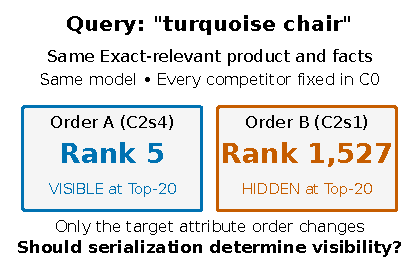
\includegraphics[width=\columnwidth]{figures/figure1_target_only.pdf}
\caption{Target-only intervention, WANDS query 162 and product 34536, MiniLM. The same Exact-relevant product crosses Top-20 with competitors fixed in C0. This differs from catalog-wide reserialization.}
\Description{Identical product facts with different attribute orders yield ranks five and 1527, with the query, model and all competitor representations fixed.}
\label{fig:example}
\end{figure}

Order instability is important, but eliminating it is not sufficient. A relevant product that is never retrieved under any representation has zero crossing instability. We therefore deepen the robustness question into a recall-first evaluation: \emph{can fixed, fact-preserving representation strategies make relevant products more reliably retrievable on queries not used for strategy selection, and at what cost?} Highest-label Recall@100 is the primary strategy outcome, with relevance effectiveness, instability, and resource costs reported alongside it.

The available intervention also matters. A merchant can change one product's text, whereas a platform can change an entire index, aggregate embeddings, or store multiple vectors per product. A target-only gain does not establish a market-wide benefit, and a platform-only method is not a merchant-deployable rewriting rule. We compare these settings explicitly and prevent multi-view retrieval from receiving extra candidate slots: all methods return the same number of unique products.

Our contribution is an empirical diagnosis and controlled strategy evaluation, not a claim to invent centroid averaging, multi-vector retrieval, or rank fusion. We ask four questions: how equivalent representations affect relevant-product inclusion; where instability concentrates after accounting for rank and input length; whether development-selected strategies transfer; and how their recall and cost compare with simply enlarging the candidate pool. We combine cross-model sensitivity, single-product interventions, rank-conditioned diagnostics, strong lexical/hybrid controls, and fixed-text reranking. Negative strategy results and the distinction between stability and useful retrieval remain central to the interpretation.
